\documentclass[a4paper,12pt]{article}
\usepackage[swedish]{babel}
\usepackage[utf8]{inputenc}
\usepackage{amsmath, amsthm, amssymb}
\usepackage{graphicx}
\usepackage{enumitem}
\usepackage[a4paper,includeheadfoot,margin=2.54cm]{geometry}
\begin{document}

\section{Dugga 3 - Fråga 3}
Låt $a = 7571$ och $b = 2147$.
\begin{enumerate}[label=\alph*)]
    \item Använd Euklides algoritm för att bestämma gcd($a$, $b$).
    \item Bestäm lcm($a$, $b$).
    \item Bestäm $m$ och $n$ så att $ma + nb = $ gcd($a$, $b$).
\end{enumerate}
\subsection*{Uträkning}
\begin{enumerate}[label=\alph*)]
    \item Euklides algoritm: 
    \begin{displaymath}
        \text{gcd}(a,~b) \rightarrow \text{gcd}(b,~a~mod~b) = \text{gcd}(b,~c)
    \end{displaymath}
    och det upprepas tills att resten blir $0$, alltså
    \begin{displaymath}
        \text{gcd}(7571,~2147)
    \end{displaymath}
    \begin{displaymath}
        \downarrow
    \end{displaymath}
    \begin{align}
        &\text{gcd}(2147,~7571~mod~2147) &=&
        7571 - (2147 \cdot (\frac{7571}{2147})) &=& 7571 - (2147 \cdot 3) &=& 1130 \label{gcd1} \\
        &\text{gcd}(1130,~2147~mod~1130) &=& 2147 - (1130 \cdot
        (\frac{2147}{1130})) &=& 2147 - (1130 \cdot 1) &=& 1017 \label{gcd2} \\
        &\text{gcd}(1017,~1130~mod~1017) &=& 1130 - (1017 \cdot (\frac{1130}{1017})) &=& 1130 - (1017 \cdot 1) &=& 113 \label{gcd3} \\
        &\text{gcd}(113,~1017~mod~113) &=& 1017 - (113 \cdot (\frac{1017}{113})) &=& 1017 - (113 \cdot 9) &=& 0
    \end{align}
    Svar: gcd$(7571,~2147) = 113$.
    \item Formel för lcm$(a,~b)$:
    \begin{displaymath}
        \text{lcm}(a,~b) = \frac{a \cdot b}{\text{gcd}(a,~b)}
    \end{displaymath}
    Jag använder mig därför av svaret från första frågan:
    \begin{align*}
        \text{lcm}(7571,~2147)  &= \frac{7571 \cdot 2147}{\text{gcd}(7571,~2147)} \\
                                &= \frac{16254937}{113} \\
                                &= 143849
    \end{align*}
    Svar: lcm$(7571,~2147) = 143849$.
    \newpage
    \item Eftersom vi vet att gcd$(a,~b) = 113$ kan vi jobba baklänges i svaren
    vi fick i första frågan för att
    hitta $m$ och $n$. Så, från \ref*{gcd3}:
    \begin{displaymath}
        113 = 1130 - 1017
    \end{displaymath}
    och från \ref*{gcd2} vet vi att:
    \begin{align*}
        113 &= 1130 - (2174 - 1130) \\
            &= 2 \cdot 1130 - 2147
    \end{align*}
    och från \ref*{gcd1} vet vi att:
    \begin{align*}
        113 &= 2 \cdot (7571 - 2147 \cdot 3) - 2147 \\
            &= 2 \cdot 7571 - 6 \cdot 2147 - 2147 \\
            &= 2 \cdot 7571 - 7 \cdot 2147
    \end{align*}
    alltså blir mitt svar:
    \begin{gather*}
        m = 2 \\
        n = -7
    \end{gather*}
\end{enumerate}
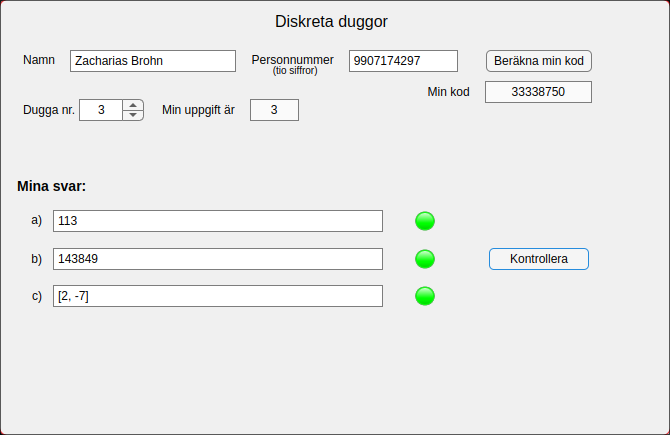
\includegraphics[width=\textwidth]{d1WK55L.png}
\end{document}